\documentclass[../main-report.tex]{subfiles}
\begin{document}

\section{Hiện thực}
\subsection{Môi trường hiện thực}
Môi trường hiện thực bao gồm:

\subsection{Các công nghệ được sử dụng}
Các công nghệ được sử dụng bao gồm:
\begin{itemize}
\item Phần giao diện người dùng: nhóm tác giả sử dụng \textbf{ReactJS/NodeJS} kết hợp \textbf{Material UI} để tạo giao diện ứng dụng web cho người dùng.
\item Phần backend được chia làm hai thành phần như sau:
\begin{itemize}
 \item Kiến trúc phi tập trung (decentralized): nhóm sử dụng ngôn ngữ solidity để xây dựng các \gls{smartcontract} kết hợp \acrshort{ipfs} để thực hiện lưu trữ các dữ liệu phi tập trung.
 \item Kiến trúc tập trung (centralized): công nghệ NodeJS kết hợp với Redis để tổ chức và tương tác với dữ liệu tập trung.
 \end{itemize} 
\end{itemize}

\subsubsection{Công nghệ ReactJS/NodeJS}

\subsubsection{Material UI framework}

\subsubsection{Cơ sở dữ liệu Redis}

\subsection{Các bước hiện thực}
\begin{itemize}
\item Bước 1
\item Bước 2
\item Bước 3
\end{itemize}

\section{Đánh giá hệ thống đã hiện thực}
\subsection{Đo lường tốc độ thực hiện giao dịch}
Để tăng tính tin cậy cho phần đánh giá dưới đây của khóa luận, nhóm tác giả đã tham khảo mô hình đánh giá và kết quả đánh giá về hiệu suất của ethereum ở các công trình khác để làm thước đo và thực hiện tương tự với mô hình đánh giá đó.

Cụ thể, công trình của tác giả Sara Rouhani và Ralph Deters \cite{rouhani2017performance} đã đo được thời gian trung bình cho mỗi \gls{transaction} là 104.609ms với Parity client và 198.9125ms với Geth. Tổng số \gls{transaction} được gửi là 2000. Hai Ethereum private \gls{blockchain} khác nhau với cùng cấu hình được thực thi bởi Parity client và Geth client được sử dụng để đo lường. Cấu hình hệ thống bao gồm 24GiB RAM và Core i7-6700 CPU. Việc gửi các \gls{transaction} được thực hiện bằng ngôn ngữ NodeJS và sau đó thu thập thời gian xử lí cho việc xác nhận các \gls{transaction}.

\subsubsection{Môi trường thực hiện đánh giá}
Nhóm tác giả thực hiện việc đánh giá này trên cấu hình máy như sau:

\begin{itemize}
\item \textbf{CPU}: Intel(R) Xeon(R) CPU E5-2673 v4 @ 2.30GHz
\item \textbf{RAM}: 2GB
\item \textbf{OS}: Ubuntu 18.04 server x64 amd
\end{itemize}

Công cụ mà nhóm tác giả sử dụng trong phần đánh giá này là \textbf{Truffle framework}\footnote{https://www.trufflesuite.com}, đây là một bộ công cụ được sử dụng để triển khai các hợp đồng thông minh hỗ trợ ngôn ngữ Solidity.

Trong phần đánh giá thời gian này, nhóm tác giả sử dụng một mạng ethereum riêng được chạy trên mạng cục bộ nhằm loại bỏ đi thời gian chờ xác nhận giao dịch thông thường trên các mạng công khai hiện tại.

\subsubsection{Phương pháp thực hiện đánh giá}
Đầu tiên nhóm tác giả thực hiện lựa chọn các hàm trong hợp đồng thông minh thường xuyên được sử dụng trong hệ thống, sau đó các hàm được chọn sẽ được hiện thực thông qua các \gls{transaction}. Các \gls{transaction} sẽ được xử lí và gửi đi bằng NodeJS, thời gian đo được tính từ lúc \gls{transaction} được tạo ra đến lúc hoàn tất \gls{transaction} đó. Với mỗi \gls{transaction}, thực hiện gửi đi tuần tự 1000 lần với cùng một input cho trước. Sau đó lấy kết quả là thời gian trung bình thực hiện cho mỗi \gls{transaction}.

Các hàm được chọn và tham số đầu vào cho mỗi hàm để đo thời gian được thể hiện ở bảng \ref{tab:listfunction-timeperform}.

\begin{table}[!ht]
\centering
\resizebox{\textwidth}{!}{%
\begin{tabular}{|l|l|l|l|}
\hline
\multicolumn{1}{|c|}{\textbf{Contract}} & \multicolumn{1}{c|}{\textbf{Hàm được chọn}} & \multicolumn{1}{c|}{\textbf{Tham số đầu vào}}                                                                                                                                                                                                                           & \multicolumn{1}{c|}{\textbf{Ghi chú}}                    \\ \hline
Wallet                                  & deposit()                                   &                                                                                                                                                                                                                                                                         & value  = $10^{15}$ gas                      \\ \hline
\multirow{3}{*}{Campaigns}              & createCampaign()                            & \begin{tabular}[c]{@{}l@{}}77760000,\\ 1000000,\\ 1,\\ {[}{]},\\ 0,\\ {[}{]},\\ '8f1ef45972ebd8ef45b2410e8a0b399181fed3d929738d2eb96baf470758a97d',\\ 'c2337a3217ffcf3b01398d83577a1c32235ceb4f481b8c7be00a055798e95d36'\end{tabular}                                   & \begin{tabular}[c]{@{}l@{}}tạo chiến dịch\\với số giai đoạn\\giải ngân $= 1$\end{tabular}            \\ \cline{2-4} 
                                        & createCampaign()                            & \begin{tabular}[c]{@{}l@{}}77760000,\\ 1000000,\\ 3,\\ {[}300000, 300000, 400000{]}\\ 2,\\ {[}0, 7200, 7200{]},\\'8f1ef45972ebd8ef45b2410e8a0b399181fed3d929738d2eb96baf470758a97d',\\ 'c2337a3217ffcf3b01398d83577a1c32235ceb4f481b8c7be00a055798e95d36'\end{tabular} & \begin{tabular}[c]{@{}l@{}}tạo chiến dịch\\với số giai đoạn\\giải ngân $> 1$\end{tabular} \\ \cline{2-4} 
                                        & donate()                                    & \begin{tabular}[c]{@{}l@{}}0,\\ 1\end{tabular}                                                                                                                                                                                                                          &                                                          \\ \hline
\end{tabular}%
}
\caption{Các hàm và tham số đầu vào được dùng để đo thời gian thực hiện giao dịch}
\label{tab:listfunction-timeperform}
\end{table}

\subsubsection{Kết quả đánh giá}
Sau khi thực hiện đánh giá thời gian, nhóm tác giả đã tổng hợp kết quả như ở bảng \ref{tab:result-timeperform}. Theo như kết quả tổng hợp được, nhóm tác giả nhận xét rằng với dữ liệu đầu vào càng nhiều (kích thước lớn) thì thời gian xử lí càng lâu.

\begin{table}[!ht]
\centering
\resizebox{\textwidth}{!}{%
\begin{tabular}{|l|l|l|l|l|}
\hline
\multicolumn{1}{|c|}{\textbf{Contract}} & \multicolumn{1}{c|}{\textbf{Hàm được chọn}} & \multicolumn{1}{c|}{\textbf{\begin{tabular}[c]{@{}c@{}}Tổng thời gian\\ 1000 lần thực hiện\\ (giây)\end{tabular}}} & \multicolumn{1}{c|}{\textbf{\begin{tabular}[c]{@{}c@{}}Thời gian trung bình\\ một giao dịch\\ (giây)\end{tabular}}} & \multicolumn{1}{c|}{\textbf{Ghi chú}}                    \\ \hline
Wallet                                  & deposit()                                   & 49.919                                                                                                             & 0.049919                                                                                                            &                                                          \\ \hline
\multirow{3}{*}{Campaigns}              & createCampaign()                            & 123.9712                                                                                                           & 0.1239712                                                                                                           & \begin{tabular}[c]{@{}l@{}}tạo chiến dịch\\với số giai đoạn\\giải ngân $= 1$\end{tabular}            \\ \cline{2-5} 
                                        & createCampaign()                            & 288.936                                                                                                            & 0.288936                                                                                                            & \begin{tabular}[c]{@{}l@{}}tạo chiến dịch\\với số giai đoạn\\giải ngân $> 1$\end{tabular} \\ \cline{2-5} 
                                        & donate()                                    & 110.999                                                                                                            & 0.110999                                                                                                            &                                                          \\ \hline
\end{tabular}%
}
\caption{Bảng kết quả đánh giá thời gian thực hiện giao dịch}
\label{tab:result-timeperform}
\end{table}

\subsection{Chi phí thực hiện các giao dịch trong hệ thống}
\subsubsection{Môi trường thực hiện đánh giá}
Nhóm tác giả thực hiện việc đo lường chi phí giao dịch trên cấu hình máy như sau:

\begin{itemize}
\item \textbf{CPU}: Intel(R) Xeon(R) CPU E5-2673 v4 @ 2.30GHz
\item \textbf{RAM}: 2GB
\item \textbf{OS}: Ubuntu 18.04 server x64 amd
\end{itemize}

Bộ công cụ \textbf{Truffle framework} kết hợp plug-in có tên là \textbf{eth-gas-reporter}\footnote{https://www.npmjs.com/package/eth-gas-reporter} được sử dụng để triển khai các hợp đồng thông minh và đo lường chi phí thực hiện. Mạng ethereum riêng chạy trên máy cục bộ được sử dụng nhằm loại bỏ đi thời gian chờ xác nhận giao dịch thông thường trên các mạng công khai hiện tại.
\subsubsection{Phương pháp thực hiện đánh giá}
Do chỉ có các hàm thực hiện ghi dữ liệu mới tốn chi phí thực hiện nên nhóm tác giả chọn ra các hàm có thao tác ghi dữ liệu, sau đó các hàm được chọn sẽ được hiện thực thông qua các \gls{transaction}. Các \gls{transaction} sẽ được xử lí và gửi đi bằng NodeJS. Sau đó thực hiện ghi lại kết quả chi phí.

Các hàm được chọn và tham số đầu vào cho mỗi hàm để đo lường chi phí được thể hiện ở bảng \ref{tab:input-cost-perform}. Các tham số đầu vào mẫu được cho là sát với thực tế khi triển khai hệ thống (độ dài từng tham số mẫu là sát với thực tế).

\begin{table}[!ht]
\centering
\resizebox{\textwidth}{!}{%
\begin{tabular}{|l|l|l|l|}
\hline
\multicolumn{1}{|c|}{\textbf{Contract}} & \multicolumn{1}{c|}{\textbf{Hàm}} & \multicolumn{1}{c|}{\textbf{Dữ liệu đầu vào}}                                                                                                                                                                                                                                                                                                                                                  & \multicolumn{1}{c|}{\textbf{Ghi chú}}                                                                \\ \hline
\multirow{2}{*}{Wallet}                 & deposit                           &                                                                                                                                                                                                                                                                                                                                                                                                & \begin{tabular}[c]{@{}l@{}}Thực hiện gửi\\ vào 2000 tokens\end{tabular}                              \\ \cline{2-4} 
                                        & withdraw                          & 1000                                                                                                                                                                                                                                                                                                                                                                                           &                                                                                                      \\ \hline
\multirow{4}{*}{Identity}               & addVerify                         & \begin{tabular}[c]{@{}l@{}}'0x93598a39777ED4B4Af3Ac7429d123Ca3bE9658C5',\\ 'AAAAB3NzaC1yc2EAAAADAQABAAAAgQCDxbho2O3XWhktz4Hwi6/61ltfk/l\\ SCqeXLufvjr6O3wh1++MmTZT+KzcO0azsKsiFJTXL7ynC06Vp1Hp9o0BK3Q/Q\\ ZTo8jRoP3XX1LBu1CLe7OeOA5P2TO/nz2mWtuxz0b11GmRrjO8YoznizlPiolL\\ kv9hoDBvwTy0JonyJ6+w=='\end{tabular}                                                                                &                                                                                                      \\ \cline{2-4} 
                                        & changePubKey                      & \begin{tabular}[c]{@{}l@{}}'0x93598a39777ED4B4Af3Ac7429d123Ca3bE9658C5',\\ 'MIGfMA0GCSqGSIb3DQEBAQUAA4GNADCBiQKBgQCMjs5j52lzXN6XX+nZ1js\\ yaBgzVBsA/JlWVux1zL0pw4GocvqPsZrIKwKsTeQycGdf3azjKRKwMga6g8fPF\\ HO+Ayh+6v33B1h+3ckWu81alwsM+Y9ADpcMret5qH2Mv9rDyWi+lmAYeUA\\ OOosAWfmgc6QJz+psSMtuGKOr08q+1wIDAQAB'\end{tabular}                                                                    &                                                                                                      \\ \cline{2-4} 
                                        & registerIdentity                  & \begin{tabular}[c]{@{}l@{}}'KLTN',\\ 'UIT-HCM, Linh Trung, Thu Duc, HCM',\\ 830550240,\\ 'QmarHSr9aSNaPSR6G9KFPbuLV9aEqJfTk1y9B8pdwqK4Rq',\\ 'frPULs0boASMCqSq1guu+jX636wkY+fzhFSRnFQi9dQuK50yzCobUIGm5b/f7\\ oGDea/NrieB5c883EpWiQdgJlO+0B43jJLAtfSfJ/mlbGX3FUPc6LAQzxlCb5FSh\\ 7+Q1E4WIUyFwLwoNdipDYFcpuXxtCsKeepjFHwGFhfupxM=',\\ '0x93598a39777ED4B4Af3Ac7429d123Ca3bE9658C5'\end{tabular} &                                                                                                      \\ \cline{2-4} 
                                        & verify                            & \begin{tabular}[c]{@{}l@{}}'0x41A418C946Fd3201b7b2b30B367De35b0c54A6ce',\\ true\end{tabular}                                                                                                                                                                                                                                                                                                   &                                                                                                      \\ \hline
\multirow{7}{*}{Campaigns}              & createCampaign                    & \begin{tabular}[c]{@{}l@{}}77760000,\\ 1000000,\\ 1,\\ {[}{]},\\ 0,\\ {[}{]},\\ '8f1ef45972ebd8ef45b2410e8a0b399181fed3d929738d2eb96baf470758a97d',\\ 'c2337a3217ffcf3b01398d83577a1c32235ceb4f481b8c7be00a055798e95d36'\end{tabular}                                                                                                                                                          & \begin{tabular}[c]{@{}l@{}}tạo chiến dịch\\ với số giai đoạn\\ giải ngân = 1\end{tabular}            \\ \cline{2-4} 
                                        & createCampaign                    & \begin{tabular}[c]{@{}l@{}}10,\\ 1000,\\ 3,\\ {[}300, 300, 400{]},\\ 0,\\ {[}{]},\\ '8f1ef45972ebd8ef45b2410e8a0b399181fed3d929738d2eb96baf470758a97d',\\ 'c2337a3217ffcf3b01398d83577a1c32235ceb4f481b8c7be00a055798e95d36'\end{tabular}                                                                                                                                                      & \begin{tabular}[c]{@{}l@{}}tạo chiến dịch\\ với số giai đoạn\\ giải ngân \textgreater 1\end{tabular} \\ \cline{2-4} 
                                        & verifyCampaign                    & \begin{tabular}[c]{@{}l@{}}1,\\ true\end{tabular}                                                                                                                                                                                                                                                                                                                                              &                                                                                                      \\ \cline{2-4} 
                                        & donate                            & \begin{tabular}[c]{@{}l@{}}1,\\ 1000\end{tabular}                                                                                                                                                                                                                                                                                                                                              &                                                                                                      \\ \cline{2-4} 
                                        & claimRefund                       & \begin{tabular}[c]{@{}l@{}}1,\\ 200\end{tabular}                                                                                                                                                                                                                                                                                                                                               &                                                                                                      \\ \cline{2-4} 
                                        & donate                            & \begin{tabular}[c]{@{}l@{}}1,\\ 200\end{tabular}                                                                                                                                                                                                                                                                                                                                               & \begin{tabular}[c]{@{}l@{}}thực hiện donate\\ lại cho đủ mục\\ tiêu chiến dịch\end{tabular}          \\ \cline{2-4} 
                                        & endCampaign                       & 1                                                                                                                                                                                                                                                                                                                                                                                              &                                                                                                      \\ \hline
Disbursement                            & vote                              & \begin{tabular}[c]{@{}l@{}}1,\\ 1,\\ true\end{tabular}                                                                                                                                                                                                                                                                                                                                         &                                                                                                      \\ \hline
\end{tabular}%
}
\caption{Các hàm và dữ liệu đầu vào được dùng để đo lường chi phí giao dịch}
\label{tab:input-cost-perform}
\end{table}

\subsubsection{Kết quả chi phí cho các giao dịch trong hệ thống}
Bảng tổng hợp chi phí cho các giao dịch được liệt kê ở bảng \ref{tab:result-cost-perform}. Kết quả màn hình khi chạy chạy công cụ đo lường chi phí được thể hiện ở hình \ref{fig:result-perform-cost-1}.

\begin{figure}[ht!]
\begin{center}
\label{fig:result-perform-cost-1}
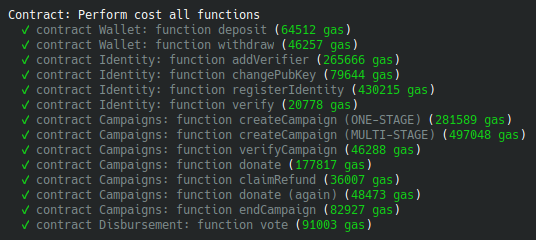
\includegraphics[scale=0.8]{result-perform-cost-1}
\caption{Ảnh chụp màn hình kết quả đo lường chi phí giao dịch}
\end{center}
\end{figure}

Công cụ đo lường còn cung cấp cho chúng ta chi phí triển khai các hợp đồng thông minh, kết quả được thể hiện ở bảng \ref{tab:result-cost-deployment}.

Một số đại lượng trong bảng kết quả:

\begin{itemize}
\item \textbf{Gas} - là một đơn vị đo lường công việc tính toán của các giao dịch hoặc hợp đồng thông minh trong mạng Ethereum.
\item \textbf{ETH} - là một đơn vị tiền tệ được sử dụng nội bộ trong mạng Ethereum. Tỉ lệ trao đổi giữa các đại lượng như sau: giá gas là 2 GWei/gas, và 1 ETH = $10^9$ GWei. Giá trị chuyển đổi giữa ETH và USD hiện tại được tham khảo trên \textbf{CoinMarketcap}\footnote{https://coinmarketcap.com} là 150.08 USD/ETH (cập nhật ngày 27/11/2019)
\end{itemize}

% Please add the following required packages to your document preamble:
% \usepackage{multirow}
\begin{table}[!ht]
\centering
\begin{tabular}{|l|l|l|l|l|}
\hline
\multicolumn{1}{|c|}{\textbf{Contract}} & \multicolumn{1}{c|}{\textbf{Hàm}} & \multicolumn{1}{c|}{\textbf{\begin{tabular}[c]{@{}c@{}}Chi phí\\ tính toán\\ (gas)\end{tabular}}} & \multicolumn{1}{c|}{\textbf{\begin{tabular}[c]{@{}c@{}}Chi phí\\ giao dịch\\ (ETH)\end{tabular}}} & \multicolumn{1}{c|}{\textbf{\begin{tabular}[c]{@{}c@{}}Chi phí\\ giao dịch\\ (USD)\end{tabular}}} \\ \hline
\multirow{2}{*}{Wallet}                 & deposit                           & 64512                                                                                             & 0.000129024                                                                                       & 0.02                                                                                              \\ \cline{2-5} 
                                        & withdraw                          & 46257                                                                                             & 0.000092514                                                                                       & 0.01                                                                                              \\ \hline
\multirow{4}{*}{Identity}               & addVerify                         & 265666                                                                                            & 0.000531332                                                                                       & 0.08                                                                                              \\ \cline{2-5} 
                                        & changePubKey                      & 79644                                                                                             & 0.000159288                                                                                       & 0.02                                                                                              \\ \cline{2-5} 
                                        & registerIdentity                  & 430215                                                                                            & 0.000860430                                                                                       & 0.13                                                                                              \\ \cline{2-5} 
                                        & verify                            & 20778                                                                                             & 0.000041556                                                                                       & 0.01                                                                                              \\ \hline
\multirow{7}{*}{Campaigns}              & createCampaign                    & 281589                                                                                            & 0.000563178                                                                                       & 0.08                                                                                              \\ \cline{2-5} 
                                        & createCampaign                    & 497048                                                                                            & 0.000994096                                                                                       & 0.15                                                                                              \\ \cline{2-5} 
                                        & verifyCampaign                    & 46288                                                                                             & 0.000092576                                                                                       & 0.01                                                                                              \\ \cline{2-5} 
                                        & donate                            & 177817                                                                                            & 0.000355634                                                                                       & 0.05                                                                                              \\ \cline{2-5} 
                                        & claimRefund                       & 36007                                                                                             & 0.000072014                                                                                       & 0.01                                                                                              \\ \cline{2-5} 
                                        & donate                            & 48473                                                                                             & 0.000096946                                                                                       & 0.01                                                                                              \\ \cline{2-5} 
                                        & endCampaign                       & 82927                                                                                             & 0.000165854                                                                                       & 0.02                                                                                              \\ \hline
Disbursement                            & vote                              & 91003                                                                                             & 0.000182006                                                                                       & 0.03                                                                                              \\ \hline
\end{tabular}
\caption{Kết quả đo lường chi phí giao dịch}
\label{tab:result-cost-perform}
\end{table}


\begin{table}[!ht]
\centering
\begin{tabular}{|l|l|l|l|}
\hline
\multicolumn{1}{|c|}{\textbf{Contract}} & \multicolumn{1}{c|}{\textbf{\begin{tabular}[c]{@{}c@{}}Chi phí\\ (gas)\end{tabular}}} & \multicolumn{1}{c|}{\textbf{\begin{tabular}[c]{@{}c@{}}Chi phí\\ (ETH)\end{tabular}}} & \multicolumn{1}{c|}{\textbf{\begin{tabular}[c]{@{}c@{}}Chi phí\\ (USD)\end{tabular}}} \\ \hline
Campaigns                               & 3447461                                                                               & 0.006894922                                                                           & 1.03                                                                                  \\ \hline
Disbursement                            & 1331555                                                                               & 0.002663110                                                                           & 0.4                                                                                   \\ \hline
Identity                                & 2401480                                                                               & 0.004802960                                                                           & 0.72                                                                                  \\ \hline
Wallet                                  & 1163284                                                                               & 0.002326568                                                                           & 0.35                                                                                  \\ \hline
\end{tabular}
\caption{Kết quả đo lường chi phí triển khai các hợp đồng}
\label{tab:result-cost-deployment}
\end{table}

\subsection{Phân tích bảo mật của hợp đồng thông minh trong hệ thống}

\end{document}